\documentclass[german]{cgspaper} % change option to 'english' to include english logo in \copyrightspace

\usepackage[ngerman]{babel} % comment out to use english in auto-generated section titles
\usepackage[utf8]{inputenc}
\usepackage[ruled]{algorithm}
\usepackage{algpseudocode}
\usepackage{url}
\usepackage{color}

\definecolor{colorMartin}{RGB}{147,83,177}
\definecolor{colorPascal}{RGB}{255,127,0}
\definecolor{colorTobias}{RGB}{160,123,46}

\newcommand{\Martin}[1]{ \textcolor{colorMartin}{TODO Martin:} #1 }
\newcommand{\Pascal}[1]{ \textcolor{colorPascal}{TODO Pascal:} #1 }
\newcommand{\Tobias}[1]{ \textcolor{colorTobias}{TODO Tobias:} #1 }

\title{Selfaware Monopoly}
\author{John Doe\\ Digital Engineering Fakultät, Hasso-Plattner-Institut \textbar{} Universität Potsdam}

% Konfiguration des Veranstaltungs-Feldes
\subject{%
    \textbf{Advanced Games of Life}\\
    Sommersemester 2018\\
    Themenstellung und Anleitung:
    XX und Prof.\ Dr.\ Jürgen Döllner}

\begin{document}

% Definition des Teasers
\teaser{
    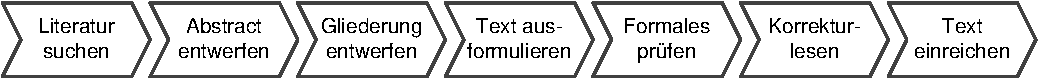
\includegraphics[width=0.9\textwidth]{graphics/prozess.pdf}
    \caption{Beispiel für einen Teaser: Schritte beim Erstellen eines fachwissenschaftlichen Beitrags. Ein Teaser dient als Blickfang schon auf der ersten Seite eines Artikels.}
    \label{fig:prozess}
}

\maketitle

%----------------------------------------------------------------
% Zusammenfassung
%----------------------------------------------------------------
\begin{abstract}
\end{abstract}

\copyrightspace % Erzeugt den Hinweis auf die Veranstaltung links unten

\section{Aufgabenstellung}
Inhaltlich erwarten wir die wissenschaftliche Auseinandersetzung mit dem bearbeiteten Seminarthema. Analog zum Abschlussvortrag empfehlen wir eine Einführung in das Thema, die Vorstellung des technischen Prototypen (Architektur, Designentscheidungen, Umsetzung), eine Diskussion über Relevanz des bearbeiteten Themas in der Gesellschaft und Vorstellen von Eigenschaften und Ergebnissen eures Prototyps. Die Struktur der Ausarbeitung und genaue Themen besprecht ihr am Besten mit eurem Betreuer.

%----------------------------------------------------------------
% Einleitung
%----------------------------------------------------------------
\section{Einleitung}

\Martin{Einführung in das Thema}

\section{Konzept}

\section{Idee}
\Martin{Konzept Idee beschreiben}

\Martin{Informationsraub beschreiben}

\Martin{Schummeln beschreiben}

\section{Ebenen des Betrügens}

\Martin{Schummelmatrix beschreiben}

\section{Vorstellung Prototyp}

\Tobias{Architektur, Designentscheidungen, Umsetzung}
\Tobias{Eigenschaften und Ergebnisse beschreiben}

\Pascal{Apis beschreiben}

\section{Diskussion}

\subsection{Apis}

\Pascal{Was könnten man als Insider in mit den Apis tun?}

\subsection{Relevanz innerhalb der Gesselschaft}

\Martin{Relevanz beschreiben}



\bibliographystyle{acmsiggraph}
\bibliography{gol-selfaware-monopoly}

\end{document}
